
\subsubsection{subfunction-oeCloseCrisis}
\label{RE-use-case-oeCloseCrisis}



the \msrcode{actCoordinator}'s goal is to declare a crisis as closed. 


\begin{usecase}
  \addheading{Use-Case Description}
  \addsingletwocolumnrow{Name}{oeCloseCrisis}
  \addsingletwocolumnrow{Scope}{system}
  \addsingletwocolumnrow{Level}{subfunction}
  

\addrowheading{Primary actor(s)}
\addnumberedsinglerow{}{\msrcode{actCoordinator[active]}}



\addrowheading{Goal(s) description}
\addsinglerow{
the \msrcode{actCoordinator}'s goal is to declare a crisis as closed. 
}

\addrowheading{Protocol condition(s)}
\addnumberedsinglerow{}{
the iCrash system has been deployed.
}

\addrowheading{Pre-condition(s)}
\addnumberedsinglerow{}{
none
}

\addrowheading{Main post-condition(s)}
\addnumberedsinglerow{}{
the crisis is know by the system to be closed.
}
\addnumberedsinglerow{}{
a message \msrcode{ieMessage(AMessage)} is sent to the \msrcode{actCoordinator} to inform him that his crisis is now considered as closed.
}


\end{usecase} 

Figure \ref{fig:lu.uni.lassy.excalibur.examples.icrash-lu.uni.lassy.excalibur.examples.icrash-RE-UCD-uc-oeCloseCrisis}
shows the use case diagram for the oeCloseCrisis subfunction use case

\begin{figure}[htbp]
\begin{center}

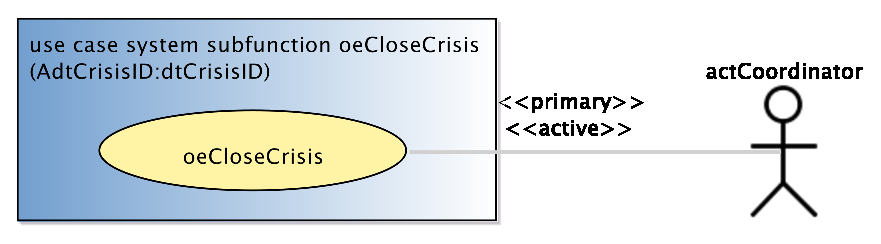
\includegraphics[
angle=0
]{./images-report-gen/appendix/lu.uni.lassy.excalibur.examples.icrash/usecase-model/subfunction/uc-oeCloseCrisis.eps}
\end{center}
\caption[lu.uni.lassy.excalibur.examples.icrash Use Case Diagram: uc-oeCloseCrisis]{ oeCloseCrisis subfunction use case}
\label{fig:lu.uni.lassy.excalibur.examples.icrash-lu.uni.lassy.excalibur.examples.icrash-RE-UCD-uc-oeCloseCrisis}
\end{figure}
\vspace{0.5cm}
